\documentclass[compress,]{beamer}

%presentation layout

\mode<presentation>
{
  \usetheme{Berlin}
  % \usecolortheme{dove}
  \setbeamercolor{structure}{bg=white,fg=black}
  \setbeamercolor{normal text}{bg=white,fg=black}
  \setbeamercolor{titlepage}{bg=white,fg=black}
  \setbeamercolor{titlelike}{bg=white,fg=black}
  \setbeamercolor{palette primary}{bg=white}
  \setbeamercolor{palette secondary}{bg=white, fg=white}
  \setbeamercolor{palette tertiary}{bg=white, fg=white}
  \setbeamercolor{palette quarternary}{bg=black}
  \setbeamercovered{transparent}
  \useinnertheme{rectangles}
  %\usefonttheme{serif}
}

\setbeamertemplate{navigation symbols}{}

%loading packages
\usepackage[ngerman]{babel}
\usepackage[T1]{fontenc}
\usepackage[utf8]{inputenc}
\usepackage{graphicx}
\usepackage{amsmath}

% vorgeplaenkel
\title[ZäPFchen-Einführung]{ZäPFchen-Einführung}

\author{Ständiger Ausschuss aller Physikfachschaften}

\institute[Zusammenkunft aller Physikfachschaften]

\date{12. Mai 2021}

\subject{ZäPFchen-Einführung}

\begin{document}

\begin{frame}
  \titlepage

  % \begin{figure}
  %   \centering
  %   \includegraphics[]{}
  % \end{figure}
\end{frame}

\section{ZäPFchen-Einführung}

%%%Folie 1


\section{Was passiert mit mir?}

\subsection{Ablauf}

\begin{frame}{Ablauf}

%  \begin{figure}
%    \centering
%    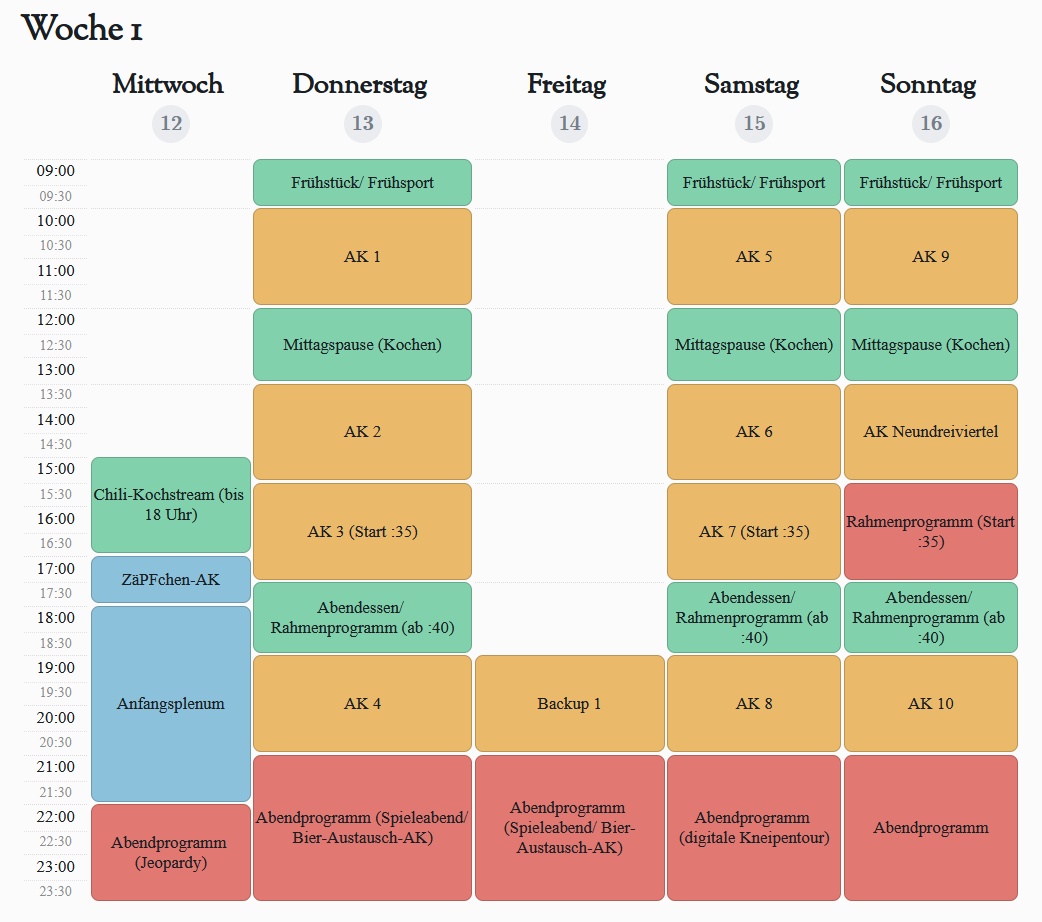
\includegraphics[scale=0.225]{OstseePlan1.png}
%
%    \caption{Viel Spaß, Essen und Unterhaltung. Dazwischen etwas Arbeit in AK...}
%  \end{figure}

\begin{figure}
   \begin{minipage}[b]{.45\linewidth} % [b] => Ausrichtung an \caption
      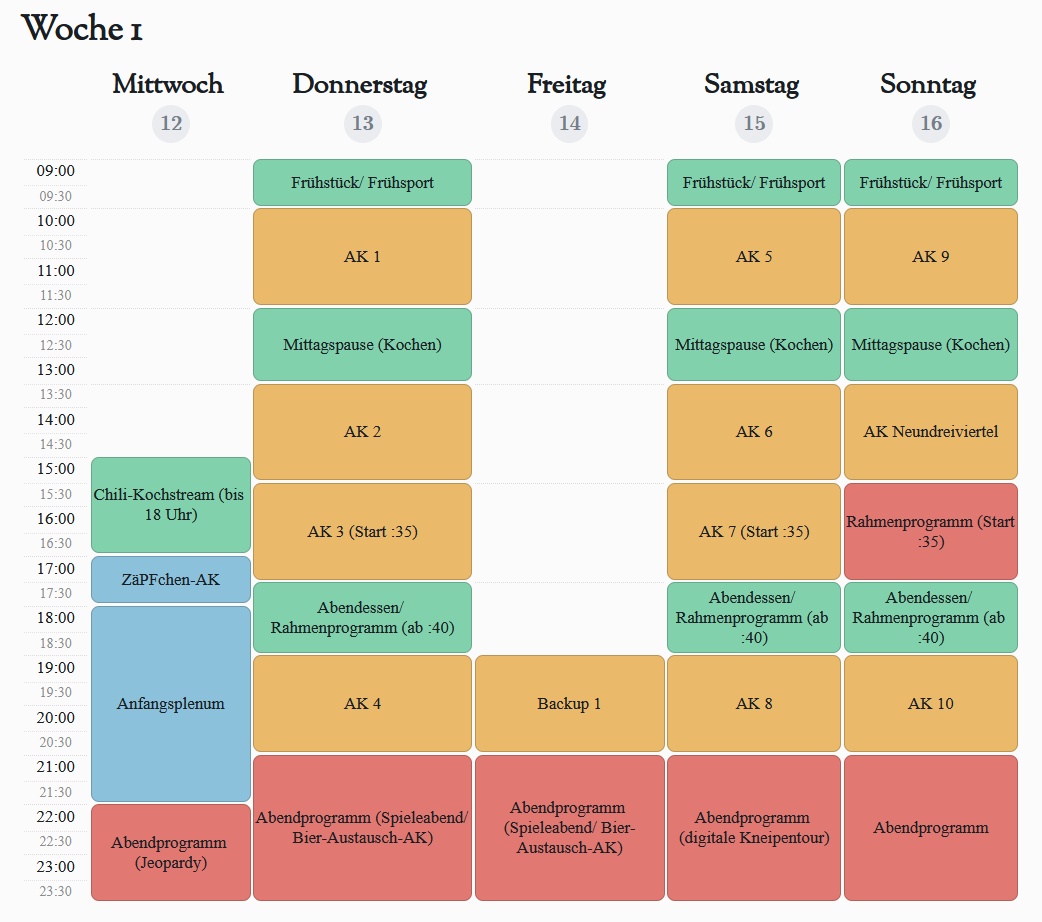
\includegraphics[width=\linewidth]{OstseePlan1.png}
      
   \end{minipage}
   \hspace{.05\linewidth}% Abstand zwischen Bilder
   \begin{minipage}[b]{.45\linewidth} % [b] => Ausrichtung an \caption
      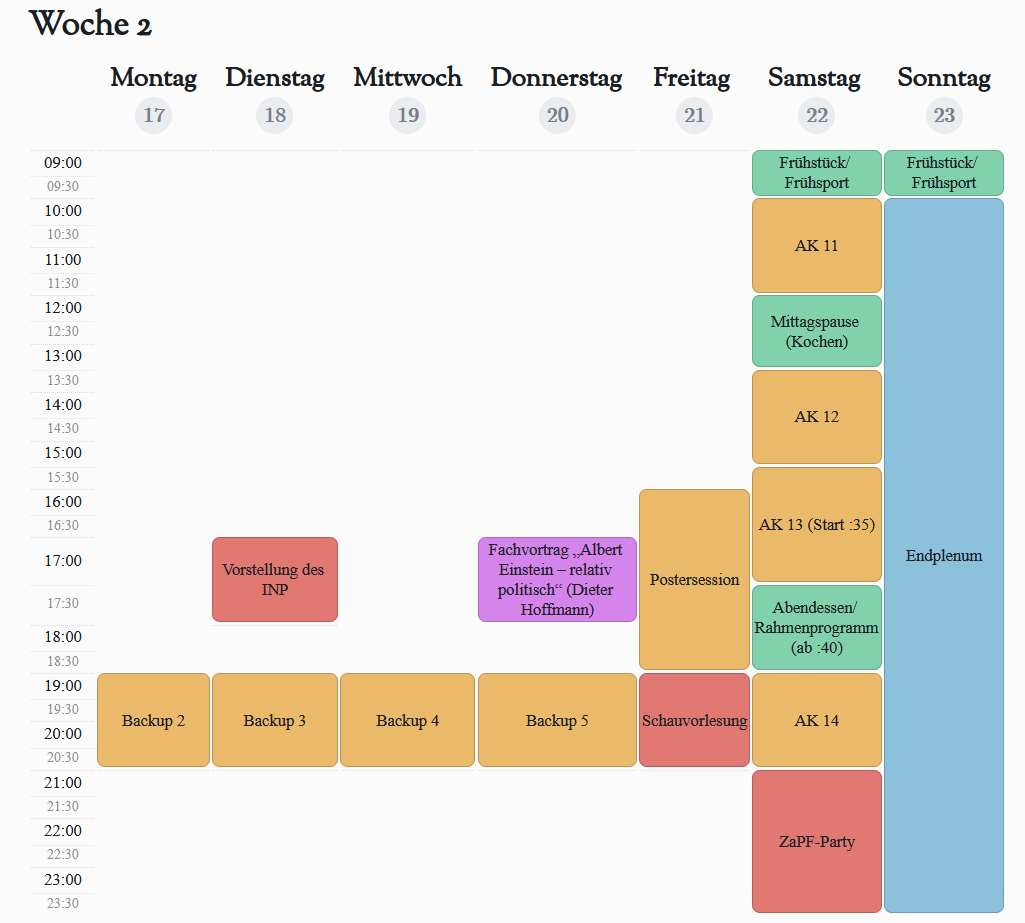
\includegraphics[width=\linewidth]{OstseePlan2.png}
      
   \end{minipage}
   \caption{Viel Spaß, Essen und Unterhaltung. Dazwischen etwas Arbeit in AK...}
\end{figure}

\end{frame}

%%%Folie 3

\subsection{BBB und ich}
\begin{frame}{BBB und ich}
  \begin{itemize}[<+->]
  \item Erster Schritt geschafft. Ihr seit hier!
  \item \textbf{Digitale Welt von Rostock erklären}
  \end{itemize}

\end{frame}


\subsection{Aufbau}

\begin{frame}{Plenum? Plenums? Plena?}

  \begin{itemize}[<+->]
  \item \textbf{Was ist es?} Das oberste beschlussfähige Gremium der ZaPF.
  \item \textbf{Wer?} Das ZaPF-Plenum sind wir alle gemeinsam.
  \item \textbf{Wann?} Anfang und Ende.
  \item \textbf{Wie?} Geschäftsordnung steht im Tagungsheft
  \item \textbf{Was passiert?} Wahlen, Abstimmungen, Vorstellen von Ergebnissen

    Ergebnisse kommen aus Arbeitskreisen, die im Anfangsplenum eingeteilt werden.
  \item Beim digitalen Plenum werden einige Wahlen digital stattfinden. Einige werden im Anschluss an die ZaPF per Briefwahl stattfinden.  
  \end{itemize}

%%%Folien 4

\end{frame}

\begin{frame}{Was ist ein Arbeitskreis?}

  \begin{itemize}[<+->]
  \item \textbf{Wieso?} Im Plenum diskutieren ist anstrengend.

    In kleine(re)n Gruppen zu sprechen ist effektiv und zeitsparend
  \item \textbf{Wann?} Zweistündige Slots an allen Tagen außer am ersten und letzten.
  \item \textbf{Wie?} 5 bis 30 Teilnehmer

    Teilweise mit Gästen, Vorträge, Workshops oder andere Formate
  \item Arten?
    \begin{itemize}[<+->]
    \item ``Normal'': Diskussionen und Austausch
    \item Austausch-AK: viele kurze Themen
    \item Folge-AK: braucht meist Vorwissen
    \item Spaß-AKs (Ausnahmen): Bier-Austausch, Fachschaftsfreundschaften
    \end{itemize}
  \end{itemize}

\end{frame}

%%%Folie 5

\subsection{ZaPF-Wiki}

\begin{frame}{Hey¸ hey, Wiki! hey, Wiki, hey!}

\begin{itemize}[<+->]
	\item ZaPF-Wiki = Arbeitsplattform
	\item Sammelt Ergebnisse von ZaPFen
	\item Bereitet ZaPFen vor
	\item Im Wiki könnt ihr euch mit euren ZaPF Account anmelden
\end{itemize}

\end{frame}

\subsection{ZaPF- Forum}

\begin{frame}{Das Forum}

\begin{itemize}[<+->]
	\item ZaPF-Forum = Austauschplattform zu einzelnen Themen und AKs
	\item ZaPF übergreifende Plattform
	\item Auch hier könnt ihr euch mit euren ZaPF Account anmelden

\end{itemize}

\end{frame}

\begin{frame}{Messengers}

\begin{itemize}[<+->]
	\item Schreibe mit ZaPFika live und in Farbe
	\item Wir folgenden Medien gibt es ZaPF Gruppen:
		\begin{itemize}
			\item Telegram
			\item Signal
		\end{itemize}
	\item Die Einladungslinks stehen in den geteilten Notizen von BBB	
\end{itemize}

\end{frame}


%\begin{frame}{Benutzerkonto erstellen}
%%  \centering
%%  \Huge{Alt + Tab}
%\begin{figure}
%\centering
%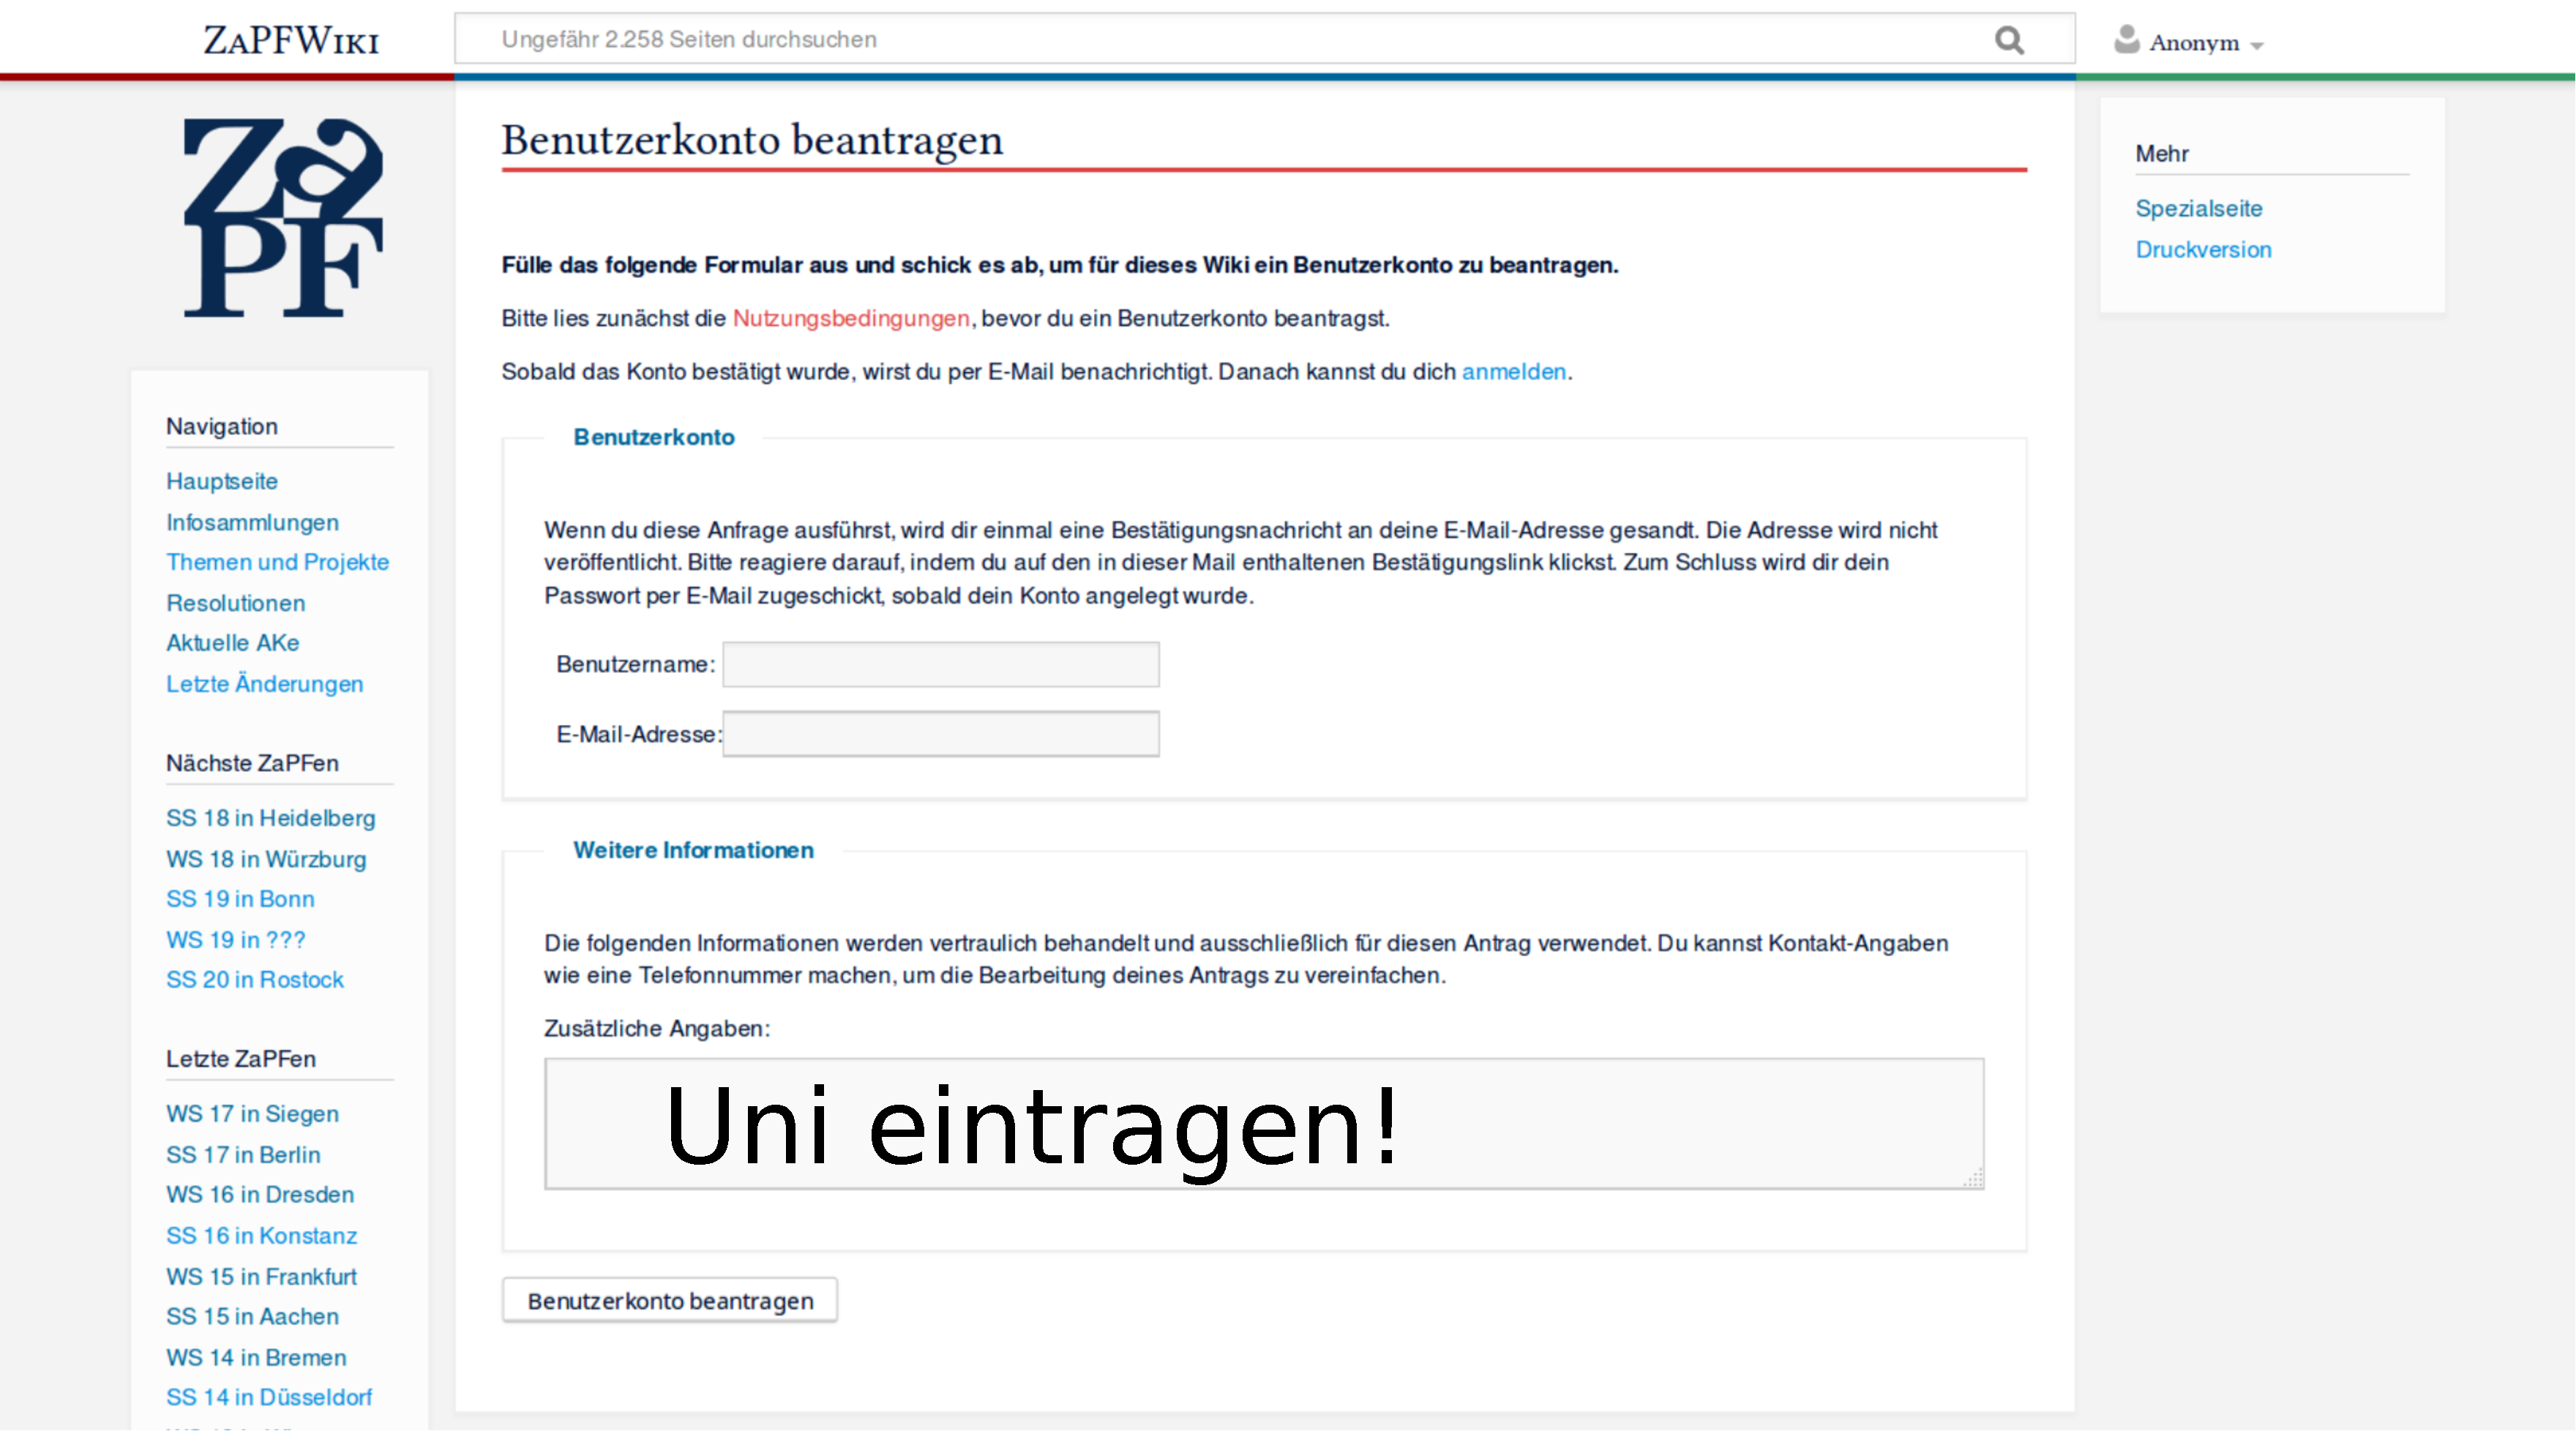
\includegraphics[scale=0.15]{ZaPFWiki_2.pdf}
%
%\caption{https://zapf.wiki/Spezial:Benutzerkonto\_beantragen}
%\end{figure}
%
%\end{frame}

%%%Folie 6


\subsection{Protokolle}

\begin{frame}{Protokolle}

  \begin{itemize}
  \item<1-> Zu jedem AK \emph{muss} ein Protokoll geschrieben werden.
  \item<2-> \textbf{Wie?} Vorlagen sind im Wiki.

  \item<3-> Speichert diese auch im Wiki ab!
  \item<3-> \textbf{Warum?}
    \begin{itemize}
    \item<4-> Weitere Arbeit an selben Themen (Folge-AKs)
    \item<5-> Fasst AKe zusammen
    \item<6-> Füllen Gedächtnislücken
    \end{itemize}
  \item<7-> Werden für die Nachwelt im Reader und im Wiki erhalten
  \end{itemize}

\end{frame}


%%% Folie 7

\subsection{Kleinigkeiten}

\begin{frame}{Kleinigkeiten}

\begin{itemize}
	\item<1-> Ja wir LIEBEN Abkürzungen, im Tagungsheft findet ihr näheres
	\item<2-> Enten sind toll
	\begin{figure}
		\centering
		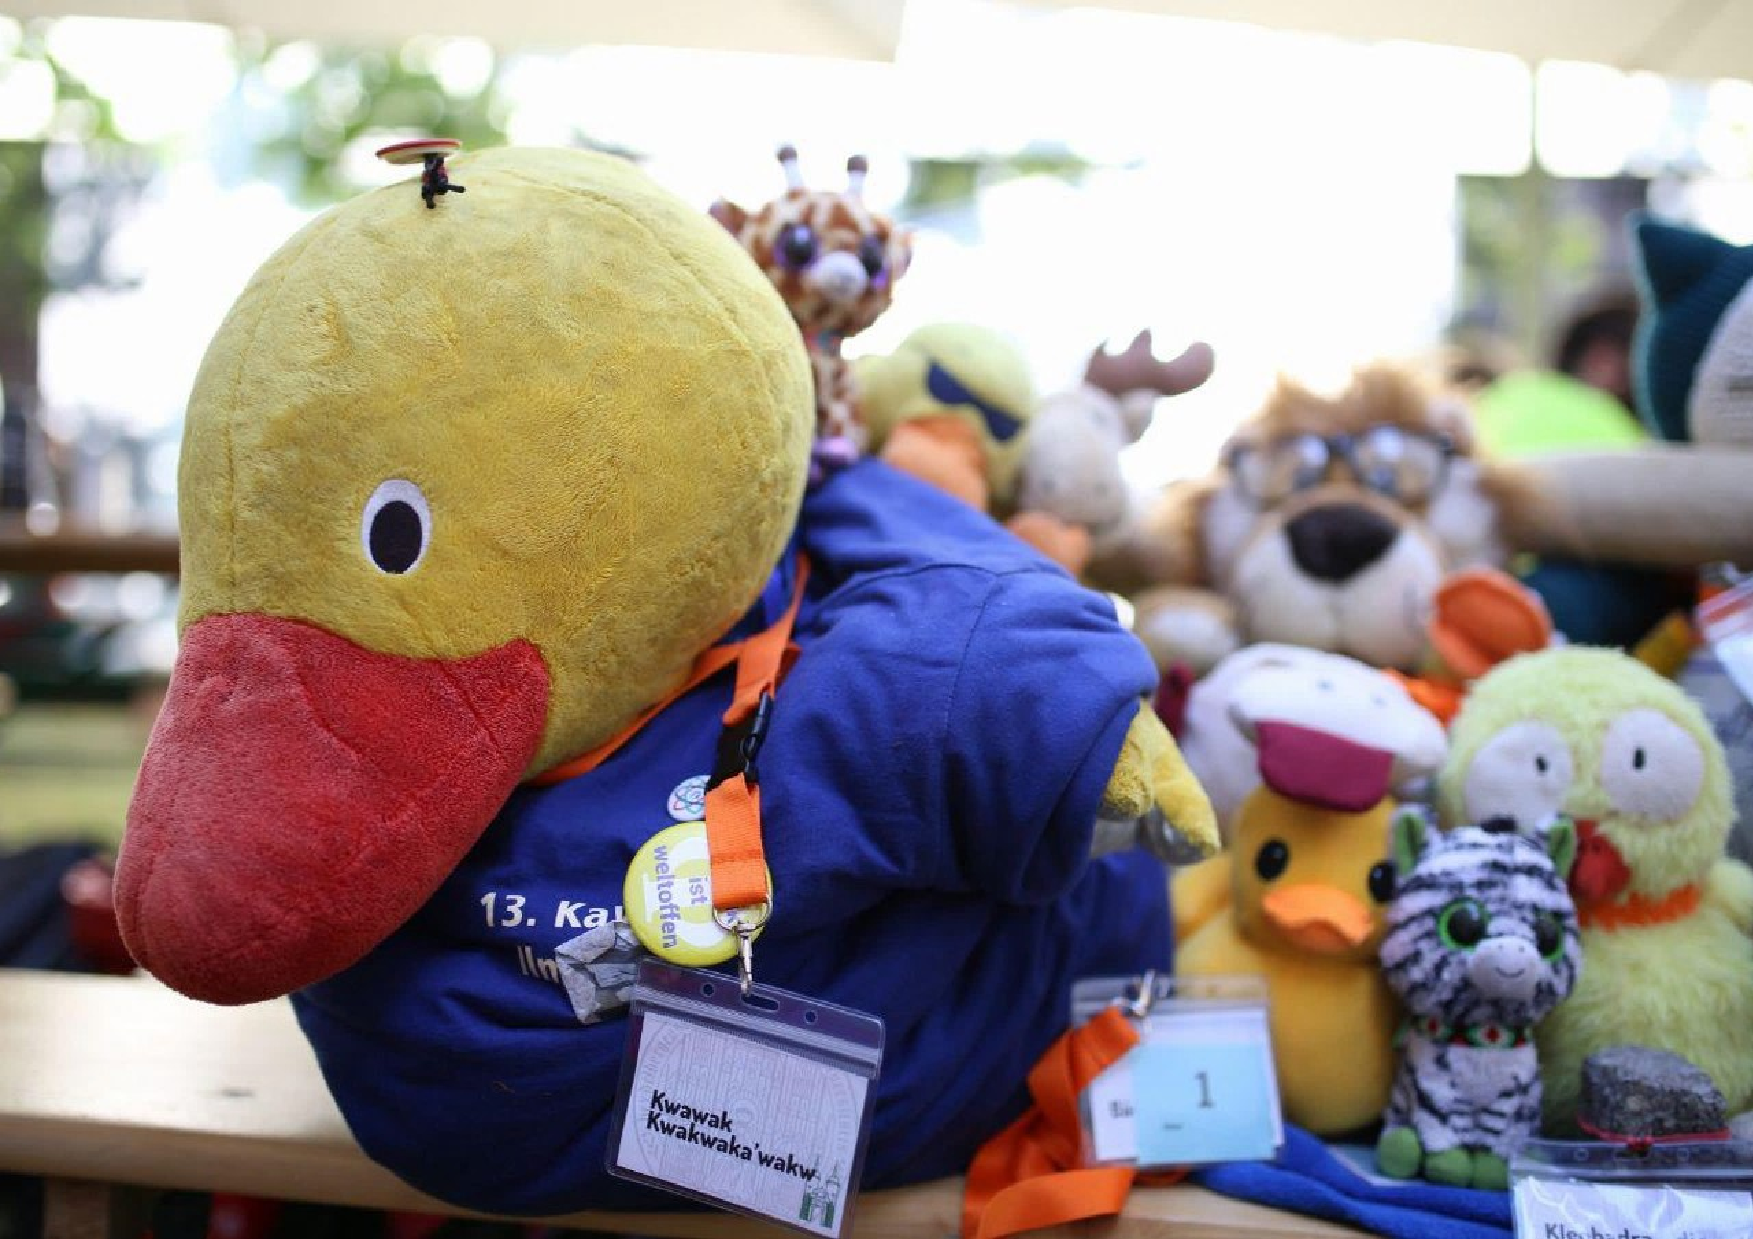
\includegraphics[scale=0.1]{Ente.pdf}
	\end{figure}
	
\end{itemize}
\end{frame}
%%% Folie 8

\section{Viel Spaß}

\begin{frame}{Viel Spaß}

Viel Spaß und fleißiges arbeiten!

\end{frame}

\end{document}

% Folgender Abschnitt nur für Emacs inklusive Auctex
%%% Local Variables: 
%%% mode: latex
%%% TeX-master: t
%%% End:
